
\documentclass[11pt,fleqn]{article}
\usepackage[margin=1in,top=1in,bottom=1in]{geometry}
\usepackage{mathtools}
\usepackage{longtable}
\usepackage{enumitem}
\usepackage{hyperref}
\usepackage[dvips]{graphics}
\usepackage[table]{xcolor}

\usepackage[normalem]{ulem}

\usepackage{multicol}
\usepackage{txfonts}
%\usepackage{amsfonts}
\usepackage{natbib}
\usepackage{gb4e}
%\usepackage{/Users/judith/Library/Latex/drs}
%\usepackage{/Users/judith/Library/Latex/avm}
\usepackage[all]{xy}
\usepackage{rotating}
\usepackage{tipa}
\usepackage{multirow}
\usepackage{authblk}


\newcommand{\foc}{$_{\mbox{\small F}}$}
\newcommand{\lp}{<_{\hspace*{-.1cm}p}}
\newcommand{\lnai}{<_{\hspace*{-.1cm}nai}}

\setlength{\parindent}{.8cm}
\setlength{\parskip}{0ex}
\setlength{\headsep}{0in}

\setlength{\bibsep}{0mm}
\bibpunct[:]{(}{)}{;}{a}{,}{,}

\newcommand{\yi}{\'{\symbol{16}}}
\newcommand{\nasi}{\~{\symbol{16}}}
\newcommand{\hina}{h\nasi na}
\newcommand{\ina}{\nasi na}
%\renewcommand{\abut}{$\supset$\hspace*{-0.07cm}$\subset$}
\newcommand{\tto}{t$_{top}$}
\newcommand{\wtop}{w$_{top}$}
\newcommand{\tc}{t$_c$}
\newcommand{\schwa}{\begin{sideways}e\end{sideways}}

% Semantic brackets
%\newcommand{\iss}[1]{\mbox{\protect\tiny \mbox{#1}}}
%\newcommand{\sem}[2]{\6#1\9$_\iss{#2}$} David's original
\newcommand{\6}{\mbox{$[\hspace*{-.6mm}[$}} 
\newcommand{\9}{\mbox{$]\hspace*{-.6mm}]$}}
\newcommand{\sem}[2]{\6#1\9$^{#2}$}

\newcommand{\semt}[2]{$\left[\hspace*{-.6mm}\left[\begin{tabular}[c]{@{}l@{}}#1\vspace*{-.5em}\end{tabular}\right]\hspace*{-.6mm}\right]\hspace*{-.6mm}^{#2}$}

%\renewcommand{\baselinestretch}{1.2}

\def\bad{{\leavevmode\llap{*}}}
\def\marginal{{\leavevmode\llap{?}}}
\def\verymarginal{{\leavevmode\llap{??}}}
\def\infelic{{\leavevmode\llap{\#}}}

\definecolor{Lighter}{gray}{.92}

\newcommand{\citepos}[1]{\citeauthor{#1}'s \citeyear{#1}}
\newcommand{\citeposs}[1]{\citeauthor{#1}'s}
\newcommand{\citetpos}[1]{\citeauthor{#1}'s (\citeyear{#1})}


\title{The information-structural source of projection variability}

\author[$\bullet$]{Judith Tonhauser}
\author[$\circ$]{David Beaver}
\author[$\triangleright$]{Judith Degen}
\affil[$\bullet$]{The Ohio State University}
\affil[$\circ$]{University of Texas at Austin}
\affil[$\triangleright$]{Stanford University}
\renewcommand\Authands{ and }

\begin{document}

\maketitle

\begin{abstract}

\end{abstract}

%\tableofcontents

%\newpage
			
\section{Introduction}

Projective content is utterance content that the speaker may be taken to be committed to even when the expression that contributes the content occurs in the syntactic scope of an entailment-canceling operator (see, e.g., \citealt{ccmg90}). The speaker of (\ref{eng1}), for instance, is taken to be committed to the content of the complement of {\em discover}, that Mike visited Alcatraz, since this content is entailed by the utterance. The so-called Family-of-Sentences variants of (\ref{eng1}) given in (\ref{eng2}a-d) do not entail this content because {\em discover} is embedded under entailment-canceling operators: negation in (\ref{eng2}a), the polar question operator in (\ref{eng2}b), the epistemic possibility modal {\em perhaps} in (\ref{eng2}c) and the antecedent of a conditional in (\ref{eng2}d). Since speakers who utter the sentences in (\ref{eng2}a-d) may nevertheless be taken to be committed to the content of the complement, this content, by virtue of being able to `project' over the entailment-canceling operators, is considered projective content. 

\begin{exe}
\ex\label{eng1}  Felipe discovered that Mike visited Alcatraz.

\ex\label{eng2}
\begin{xlist} 
\ex Felipe didn't discover that Mike visited Alcatraz.
\ex Did Felipe discover that Mike visited Alcatraz?
\ex Perhaps Felipe discovered that Mike visited Alcatraz.
\ex If Felipe discovered that Mike visited Alcatraz, he'll get mad.
\end{xlist}
\end{exe}

Why does projective content project? According to mainstream `conventionalist' approaches, projective content projects because it is conventionally specified to do so, for instance, by being required to be entailed by or satisfied in the common ground of the interlocutors (e.g., \citealt{heim83,vds92,geurts99}). On such approaches, the lexical entry of {\em discover} specifies that the content of its clausal complement is required to be entailed by or satisfied in the common ground of the interlocutors, thereby ensuring that the speaker is taken to be committed to the content. Since conventionalist approaches only distinguish projective and non-projective content, such approaches are challenged by the long-standing observation that some projective content projects less robustly than other such content. In the early 1970s already, \citet{karttunen71b} pointed out that the content of the complement of {\em regret} in (\ref{semi-factive}a) is more robustly projective than the content of the complement of {\em discover} in (\ref{semi-factive}b); following \citealt{karttunen71b}, predicates like {\em discover} have since been referred to as `semi-factive', in contrast to their `factive' counterparts like {\em regret} (and `non-factive' predicates like {\em believe}). In \citealt{schlenker10}, the predicate {\em announce} was referred to as a `part-time trigger' because the content of its complement may, but often does not, project.

\begin{exe}
\ex\label{semi-factive}
\begin{xlist}
\ex John didn't discover that he had not told the truth.  
\ex John didn't regret that he had not told the truth.
\hfill (\citealt[63]{karttunen71b})

\end{xlist}
\end{exe}

Similarly, \citet[432]{simons01} noted, partially based on examples from \citealt{ccmg90} and \citealt{geurts94}, that the projection of ``some -- but crucially, not all'' projective content to the common ground of the interlocutors may be suppressed in explicit ignorance contexts. Example (\ref{hardsoft}a), for instance, shows that the projective content of {\em win} in the antecedent of the conditional, that John participated in the race, need not be part of the common ground of the interlocutors, i.e., need not project. On the other hand, the existential implication of the cleft in (\ref{hardsoft}b), that there is an individual who read the letter, must be part of the common ground of the interlocutors, i.e., must project. Expressions like {\em win} are referred to as `soft triggers', in contrast to `hard triggers', like the cleft.

\begin{exe}
\ex\label{hardsoft}
\begin{xlist}

\ex I have no idea whether John ended up participating in the Road Race yesterday. But if he won it, then he has more victories than anyone else in history. \hfill (\citealt[39]{abusch10})

\ex\infelic I have no idea whether anyone read that letter. But if it is John
who read it, let's ask him to be discreet about the content. \hfill (\citealt[40]{abusch10})

\end{xlist}
\end{exe}

Experimental research has also provided preliminary evidence for projection variability. \citet{xue-onea11} observed that the content of the complement of German {\em wissen} `know' is less projective than the content of the complement of {\em erfahren} `find out', both of which are less projective than the relevant projective contents of sentences with {\em auch} `too' (that a parallel event is contextually salient) and {\em wieder} `again' (that the relevant event has happened before). Similarly, \citet{smith-hall11} found that the projective contents of {\em win} and {\em know} are less projective than the content implication of English definite noun phrases (e.g., for {\em the queen}, that the referent is a queen). Interestingly, they also found that the existential implication of cleft sentences, considered a hard trigger, was (numerically) less projective than the relevant contents of the soft triggers {\em win} and {\em know}. Thus, the sparse experimental evidence confirms some but not all of the intuitions about projection variability reported in the literature.

Observations about projection variability challenge conventionalist approaches to projection because such approaches do not offer an explanation for why some projective content seems to project less robustly than other such content. After all, under such approaches, any expression that contributes projective content lexically specifies that the relevant content is required to be entailed by or satisfied in the common ground of the interlocutors. The lexical specifications of expressions like {\em regret, discover, win}, clefts and definite noun phrases thereby predict that their relevant contents can project, but do not predict differences in how robustly the contents project.\footnote{\citet{schlenker10} says his analysis predicts this; read!} Referring to triggers of projective content as `semi-factive' or `soft', as opposed to `factive' or `hard', serves to remind of projection variability but does not address the challenge that this variability poses for conventionalist approaches to projection.

One possible explanation for projection variability is that the projectivity of such content derives from a property that projective content shares, but shares to varying degrees. \citet{brst-salt10} proposed that this property is `at-issueness', i.e., the ability of content to address the Question Under Discussion (QUD; e.g., \citealt{roberts12}). Specifically, Simons and her colleagues proposed that utterance content projects if and only if it is not at-issue with respect to the QUD addressed by the utterance. This proposal predicts, for instance, that the content of non-restrictive relative clauses projects more robustly, by virtue of being not at-issue (\citealt{potts05}), than the content of the complement of {\em discover}, which can be at-issue (\citealt{simons07}).  In (\ref{nrrc}a), for instance, the content of the non-restrictive relative clause in B's utterance cannot be used to address A's question, and hence is not at-issue, in contrast to the main clause content of B's utterance, as shown in (\ref{nrrc}b). The content of the complement of {\em discover} in B's utterance in (\ref{discover}a), on the other hand, can address A's question, and hence can be at-issue, but it can also be not at-issue, as shown in (\ref{discover}b), where it does not address A's question.\footnote{\citet{syrett-koev2015} show that the content of non-restrictive relative clauses can be the target of direct denial, which may be taken to suggest that this content can be at-issue. We return to this matter in section \ref{s3}.}

\begin{exe}
\ex\label{nrrc}
\begin{xlist}
\ex
\begin{xlist}
\exi{A:} Did Mike visit Alcatraz?
\exi{B:} \infelic Mike, who visited Alcatraz, is interested in the history of prisons.
\end{xlist}


\ex
\begin{xlist}
\exi{A:} What is Mike interested in?
\exi{B:} Mike, who visited Alcatraz, is interested in the history of prisons.
\end{xlist}


\end{xlist}

\ex\label{discover}
\begin{xlist}
\ex
\begin{xlist}
\exi{A:} Where was Harriet yesterday?
\exi{B:} Henry discovered that she had a job interview at Princeton. \hfill (\citealt[1035]{simons07})
\end{xlist}
\ex
\begin{xlist}
\exi{A:} Why is Henry in such a bad mood?
\exi{B:} He discovered that Harriet had a job interview at Princeton. 
\end{xlist}
\end{xlist}
\end{exe}

This paper has two goals, which are explored on the basis of two pairs of experiments. The first goal (Experiments 1a and 1b) is to empirically explore projection variability for a broad range of projective content, in order to better understand the extent to which projection variability presents a challenge for conventionalist approaches to projection. The second goal (addressed through Experiments 1a and 1b, as well as 2a and 2b) is to test the proposal put forth in \citealt{brst-salt10}, that the projectivity of utterance content is influenced by at-issueness, i.e., the information-structural status of such content. These two goals jointly serve to assess the empirical adequacy of conventionalist and \citetpos{brst-salt10} approaches to projection and projection variability.

In pursuing our first goal, we expand and improve on previous experimental research. In \citealt{xue-onea11} and \citealt{smith-hall11}, projection variability was explored for 4 German and 6 English expressions that contribute projective content, respectively. Experiments 1a and 1b significantly broaden our understanding of projection variability by considering the projective content of 19 expressions (whose properties are introduced in section \ref{s2}). Our experiments also take into consideration that the prior plausibility of content may influence projection: a speaker might, for instance, be more likely to be taken to be committed to the content that Alexander flew to New York than to the content that Alexander flew to the moon, simply because people are more likely to fly to New York than the moon. In other words, the content of the projective content of an expression\footnote{In this paper, we use `content' to refer to the content of an expression and `projective content' to refer to an abstract characterization of the projective content of an expression. For instance, in B's utterance in (\ref{discover}a), the relevant expression is {\em discover}, the projective content is the content of its clausal complement, and the content (of the projective content) is that Harriet had a job interview at Princeton.} may matter for how robustly the projective content is taken to be a commitment of the speaker (and how likely the projective content is to address the QUD). The projective content of the 6 expressions explored in \citealt{smith-hall11} was only instantiated by one content each and a distinct content instantiated each projective content; similarly, the projective content of the 4 expressions explored in \citealt{xue-onea11} was instantiated by three distinct contents each. Our experiments, in contrast, included a total of 37 contents and the projective content of each expression was instantiated by up to 20 contents. Furthermore, to facilitate comparison across the different projective contents (and the expressions that contribute them), the projective contents contributed by distinct expressions were instantiated with the same contents: overall, each of the 37 contents instantiated up to 12 projective contents.

Our second goal, to explore the hypothesis that the information-structural status of projective content influences its projectivity, also builds on previous experimental work. 
 Using a direct dissent diagnostic for at-issueness, \citet{amaral-etal11} found that speakers of British English judged direct dissent with the projective content of {\em only} (the prejacent) to be more acceptable than direct dissent with the projective content of {\em continue} and {\em stop} (the pre- and post-states, respectively). These findings suggest that the prejacent of {\em only} is more at-issue than the post- and pre-state content of {\em continue} and {\em stop}. (See also \citealt{cummins-etal2012}.) \citet{xue-onea11} found that speakers of German were more likely to directly dissent with the content of the complement of {\em wissen} `know' than with the content of the complement of {\em erfahren} `find out' and, in turn, more likely to directly dissent with these contents than with projective contents of {\em auch} `too' and {\em wieder} again'. These results suggest that the content of the complement of {\em wissen} `know' is more at-issue than the content of the complement of {\em erfahren} `find out', which in turn are comparatively more at-issue than the relevant contents of {\em auch} `too' and {\em wieder} again'. Interestingly, comparing the relative projectivity and not-at-issueness 
of the contents across their two experiments, \citet[180]{xue-onea11} point to ``a clear correlation between projection and not-at-issueness'', in line with the proposal made by \citealt{brst-salt10}. Our Experiments 1a and 1b improve on \citetpos{xue-onea11} study by exploring the projectivity and the not-at-issueness of projective content as within-item and within-participant factors. This experiment design allows us to quantify the influence of not-at-issueness on the projectivity of utterance content but also to assess item- and participant-variability. Since different diagnostics have been used in the literature to diagnose (not-)at-issueness (for discussion, see, e.g., \citealt{tonhauser-sula6} and section \ref{s2}), the second pair of experiments, Experiments 2a and 2b, explore the not-at-issueness of the contents of the first pair of experiments, Experiments 1a and 1b, using a different diagnostic for at-issueness. The results of the two pairs of experiments thus also allow for a comparison of two diagnostics for at-issueness.

The paper proceeds as follows. In section \ref{s2}, we introduce properties of the projective contents explored in this paper and our assumptions about at-issueness. Section \ref{s3} addresses the two goals of the paper on the basis of Experiments 1a and 1b, and our investigation of the second goal is extended in section \ref{s4} on the basis of Experiments 2a and 2b. In section \ref{s4}, we discuss the implications of our findings for conventionalist and \citetpos{brst-salt10} approaches to projection and projection variability.

\section{Properties of the projective contents explored in the experiments}\label{s2}

This section introduces properties of the projective contents explored in the two pairs of experiments. These projective contents are contributed by 19 expressions, henceforth referred to as `triggers', but without making any commitment to these expressions conventionally specifying the projectivity of the relevant content. 

The projective contents were selected so as to include a syntactically heterogeneous set of triggers in Experiments 1a and to zoom in on a particular syntactic type of trigger, namely attitude predicates, in Experiment 1b. Experiments 2a and 2b explored not-at-issueness for the same trigger/projective content pairs as Experiments 1a and 1b, respectively. The 9 trigger/projective content pairs explored in Experiments 1a and 2a are given in (\ref{pairs1a2a}), together with examples the clarify the projective content explored. {\bf JT: YES? USEFUL?} The 12 trigger/projective content pairs explored in Experiments 1b and 2b are given in (\ref{pairs1b2b}): since the projective content of the attitude predicates {\em annoyed} and {\em discover} were explored across all four experiments, a total number of 19 trigger/projective content pairs were explored.

\begin{exe}
\ex\label{pairs1a2a} {\bf Trigger/projective content pairs in Experiments 1a and 2a}

\begin{enumerate}[itemsep=-.5mm]

\item Sentence-medial non-restrictive relative clauses / content of the NRRC
\\ e.g., {\em Martha, who has a new BMW, drives fast}; content: `Martha has a new BMW'

\item Sentence-medial nominal appositives / appositive content
\\ e.g., {\em Martha's new car, a BMW, was expensive}; content: `Martha has a BMW'


\item Posessive noun phrases / possession implication
\\ e.g., {\em Martha's new car is a BMW}; possession implication: `Martha has a new car'

\item {\em annoyed} / content of the clausal complement
\\ e.g., {\em Martha's neighbor was annoyed that Martha has a new BMW}; content: `Martha has a new BMW'

\item {\em discover} / content of the clausal complement
\\ e.g., {\em Mary discovered that her daughter has been biting her nails}; content: `Mary's daughter has been biting her nails'

\item {\em know} / content of the clausal complement
\\ e.g., {\em Billy knows that Martha has a new BMW}; content: `Martha has a new BMW'

\item {\em only} / prejacent
\\ e.g., {\em Martha only likes blueberries}; prejacent: `Martha likes blueberries'

\item {\em stop} / pre-state implication
\\ e.g., {\em Martha stopped smoking}; pre-state implication: `Martha smoked in the past'

\item {\em stupid} / prejacent
\\ e.g., {\em Martha was stupid to buy that TV}; prejacent: Martha bought that TV

\end{enumerate}


\ex\label{pairs1b2b} {\bf Trigger/projective content pairs in Experiments 1b and 2b}

\begin{enumerate}[itemsep=-.5mm]

\item {\em be amused} / content of the clausal complement

\item {\em be annoyed} / content of the clausal complement

\item {\em know} / content of the clausal complement

\item {\em be aware} / content of the clausal complement

\item {\em see} / content of the clausal complement

\item {\em discover} / content of the clausal complement

\item {\em find out} / content of the clausal complement

\item {\em realize} / content of the clausal complement

\item {\em learn} / content of the clausal complement

\item {\em establish} / content of the clausal complement

\item {\em confess} / content of the clausal complement

\item {\em reveal} / content of the clausal complement

\end{enumerate}

\end{exe}

The 19 trigger/projective content pairs explored in the experiments share some properties but also differ along lines identified in the theoretical literature:

\paragraph{Projectivity} Obviously, the 19 projective contents share the property of being projective, i.e., being able to be taken to be a commitment of the speaker. The 9 projective contents in Experiments 1a and 2a include ones that have been reported to project robustly, such as the content of non-restrictive relative clauses, nominal appositives and of the emotive `factive' predicate {\em annoyed}, as well as projective contents that have been reported to project less robustly, including the prejacent of {\em only}, the pre-state implication of {\em stop} and the complement of the cognitive `semi-factive' predicate {\em discover}. 

The 12 triggers included in Experiments 1b and 2b were chosen to include different types of attitudes, namely emotive `factive' predicates ({\em be amused, be annoyed}), cognitive `factives' predicates ({\em know, be aware}), sensory `factives' predicates ({\em see}), cognitive `semi-factives' predicates ({\em discover, find out, realize, learn, establish}) and communication `semi-factives' ({\em confess, reveal}).

\paragraph{Strong Contextual Felicity} A property that the 19 trigger/projective content pairs share is that they do not impose a Strong Contextual Felicity constraint (\citealt{brst-lang11}). This constraint distinguishes projective content based on whether the content is required to be part of the common ground of interlocutors prior to utterance of the expressions that contributes the content. Consider the pronoun {\em they}, which contributes the projective content that there is a uniquely salient plurality of individuals (to which the pronoun refers). Use of {\em they} in (\ref{scf}) is judged to be unacceptable because the projective content of the pronoun is not part of the common ground of the interlocutors, i.e., the context does not entail the existence of a uniquely salient plurality of individuals to which the pronoun could refer. Thus, this projective content of the pronoun has a Strong Contextual Felicity constraint. Other projective content triggers that impose a Strong Contextual Felicity constraint include {\em too} (there is a salient alternative proposition) and the deictic implication of demonstratives (see \citealt{brst-lang11}).

\begin{exe}
\ex\label{scf} Context: At a bus stop in San Francisco, a woman approaches another woman, with no other people are around, and asks: \\ \#Did they visit Alcatraz?
\end{exe}

The 19 trigger/projective content pairs selected for the experiments in this paper do not impose a Strong Contextual Felicity constraint: B's utterance in (\ref{nrrc}b), for instance, is acceptable even if A did not previously know the content of the non-restrictive relative clause, that Mike visited Alcatraz.\footnote{In fact, as discussed in \citealt{potts05}, appositive content like that of non-restrictive relative clauses is typically required to provide new information.} Since trigger/projective content pairs that impose a Strong Contextual Felicity constraint are only judged to be acceptable in contexts in which the projective content is entailed, including such trigger/projective content pairs in the experiments would have meant that different stimuli would have needed to be presented in different contexts, namely ones that entail the relevant contents. Since the projectivity and not-at-issueness of projective content is sensitive to context (see, e.g., the examples in (\ref{hardsoft}), the experiments were limited to trigger/projective content pairs that do not impose a Strong Contextual Felicity constraint, which allowed all of the stimuli to be presented in the same (minimal) contexts.\footnote{Crucially, the minimal contexts in which the stimuli were presented do not plausibly allow for the projective contents to be locally accommodated (\citealt{heim83,vds92}) and hence allow us to make a case against conventionalist approaches to projection and projection variability. We return to this in section \ref{s3}.}

\paragraph{Obligatory Local Effect} \citetpos{brst-lang11} Obligatory Local Effect property distinguishes projective content based on whether the content is obligatorily contributed to an attitude holder's belief state when the expression that contributes the content occurs in the complement of a belief-predicate. Most but not all of the 19 projective contents explored in the experiments have this property. Consider the examples in (\ref{ole}), where the non-restrictive relative clause and the complement of {\em discover} occur as part of the complement clause of {\em believe}. The attitude holder Sarah need not be committed to the projective content contributed by the non-restrictive relative clause, as shown by the acceptability of the continuation ({\em \ldots but she doesn't know that Mike visited Alcatraz}), but she must be committed to the projective content contributed by the complement of {\em discover}, as shown by the unacceptability of the same continuation. Thus, the content of NRRCs does not have Obligatory Local Effect (and neither does the projective content of appositives or of possessive noun phrases), whereas the content of {\em discover} does have Obligatory Local Effect (as do all remaning projective contents listed in (\ref{pairs1a2a}) and (\ref{pairs1b2b})).

\begin{exe}
\ex\label{ole}
\begin{xlist}
\ex Sarah believes that Mike, who visited Alcatraz, is interested in the history of prisons, \ldots but she doesn't know that Mike visited Alcatraz.

\ex Sarah believes that Felipe discovered that Mike visited Alcatraz, \ldots \#but she doesn't know that Mike visited Alcatraz. 

\end{xlist}
\end{exe}

Since the trigger/projective content pairs for Experiments 1a and 2a were chosen so as to include a diverse range of trigger/projective content pairs, these experiments include trigger/projective content pairs that do have Obligatory Local Effect as well as ones that don't. 

\section{Experiments 1a and 1b}\label{s3}

The two experiments reported on in this section were designed to explore projection variability and the correlation of projectivity and not-at-issueness for a wide range of expressions contributing projective content. In both experiments the relevant expressions were embedded in polar questions and gradient ratings about the projectivity and not-at-issueness of the relevant contents were collected. {\bf Either give example here or just leave this out. Too abstract. Can you foreshadow more what’s going to happen in the experiments?}

\subsection{Experiment 1a} 

Experiment 1a explored the appositive content of nominal appositives and non-restrictive relative clauses, the possession implication of possessive noun phrases, the prejacent of sentences with {\em only} and {\em stupid}, the pre-state of sentences with {\em stop} and the contents of the clausal complements of {\em discover, know} and {\em be annoyed}. {\bf How were these chosen?}

\subsubsection{Methods}\label{s-methods-1a}

\paragraph{Participants.} 250 participants with U.S.\ IP addresses and at least 97\% of previous HITs approved were recruited on Amazon's Mechanical Turk platform. They were paid \$1 for participating in the experiment. 

\paragraph{Procedure.} Participants were told to imagine that they are at a party and, upon walking into the kitchen, overhear somebody ask another person a question. Participants were then presented twice with their 15 polar question stimuli (for a total of 30 polar question stimuli): {\bf JD: was this a blocked design?} in one half of the experiment, participants responded to `certain that' questions (assessing projectivity) about the 15 stimuli in a random order (see, e.g., (\ref{stim}a)); in the other half, participants responded to `asking whether' questions (assessing not-at-issueness) about the same 15 stimuli in a (different) random order (see, e.g., (\ref{stim}b)). Which type of question a participant responded to first was decided at random. The `certain that' question assessed the extent to which the participant took the speaker (e.g., `Patrick' in (\ref{stim})) to be committed to the relevant content, i.e., the extent to which the content projects from the polar question. The `asking whether' question assessed the extent to which the participant took the speaker to be asking about the relevant content, i.e., the extent to which the content was at-issue in the speaker's polar question. (See, e.g., \citealt[731]{amaral-etal07} and \citealt{tonhauser-sula6} for earlier uses of this diagnostic for at-issueness.)

\begin{exe}

\ex\label{stim} Patrick asks: {\em Was Martha's new car, a BMW, expensive?} (= (\ref{examples-1a}b))

\begin{xlist}
\ex `certain that' question: Is Patrick certain that Martha's new car is a BMW?

\ex `asking whether' question: Is Patrick asking whether Martha's new car is a BMW?

\end{xlist}

\end{exe}

Participants read the polar question stimuli as well as the corresponding questions and gave their responses on a slider marked `no' at one end and `yes' at the other, as shown in Figure \ref{f-trial-exp1}.  


\begin{figure}[!h]
\begin{center}
\fbox{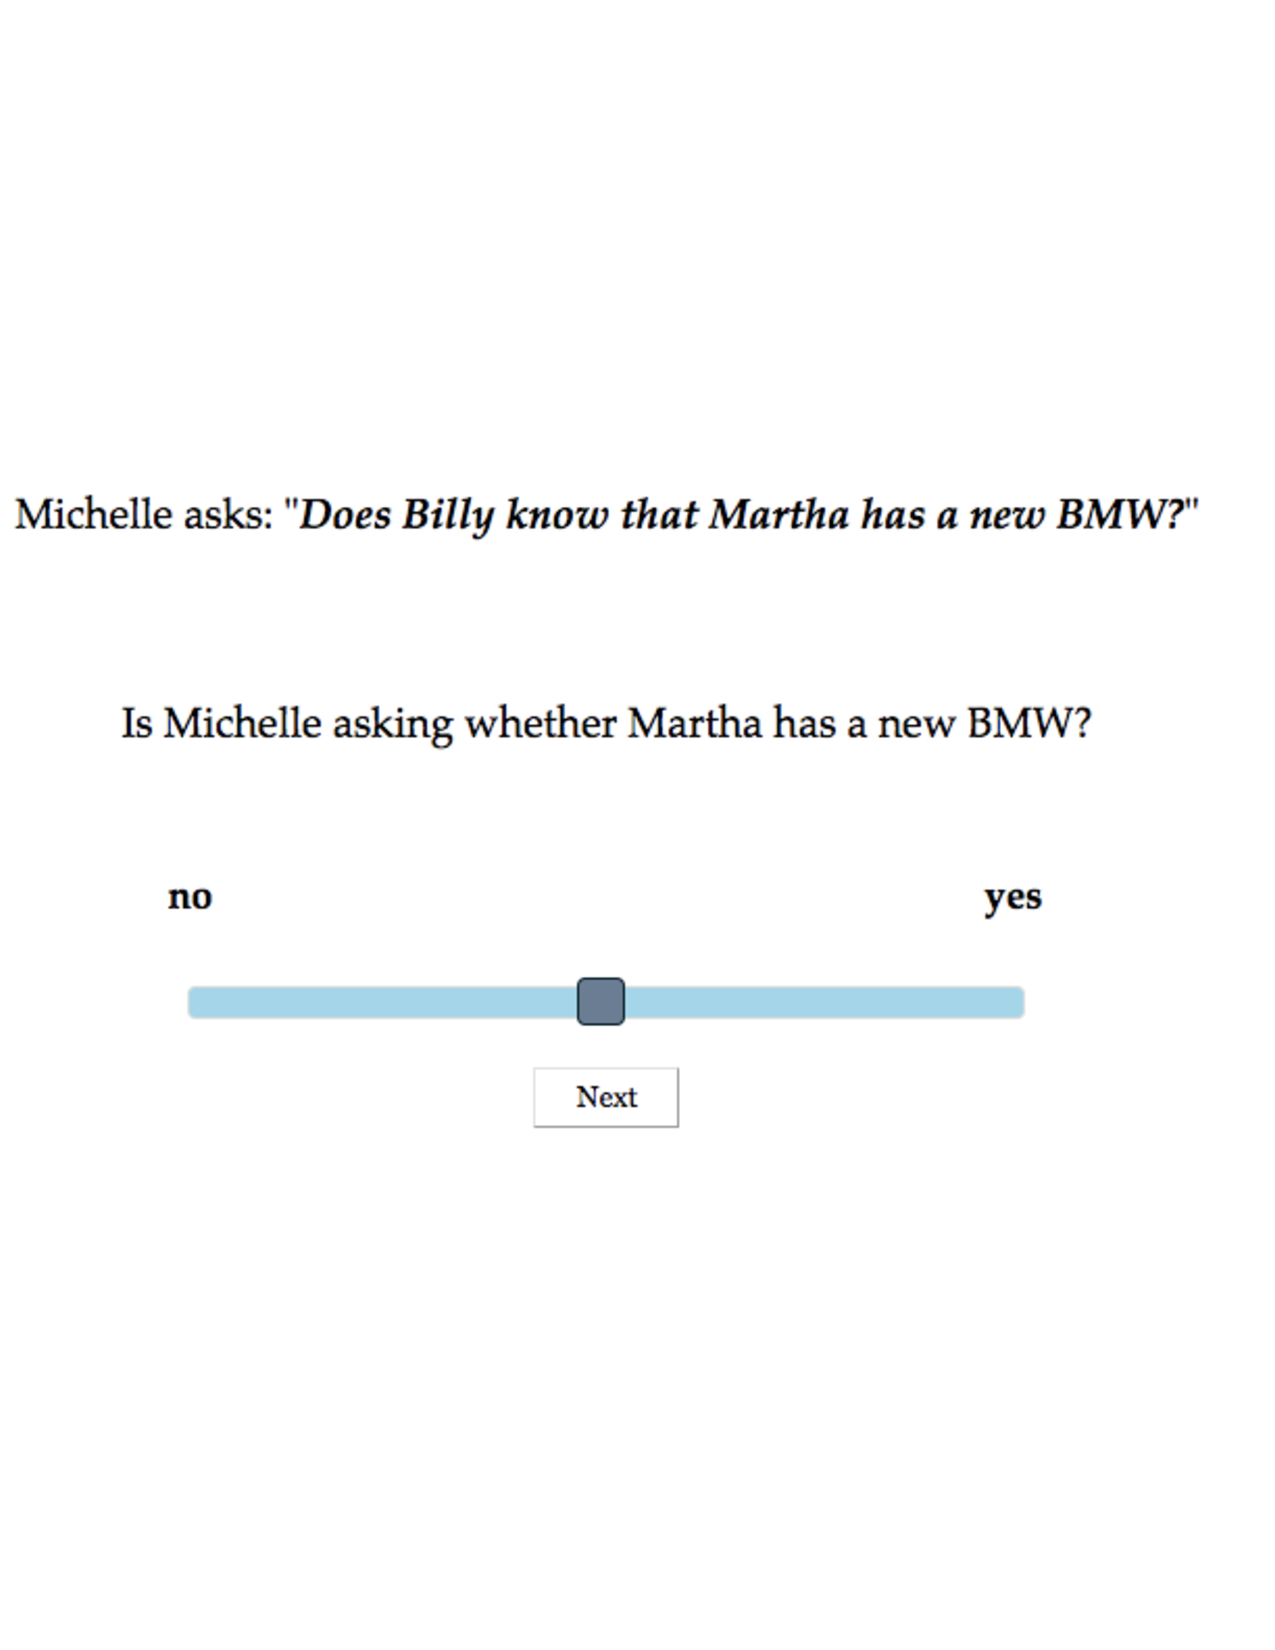
\includegraphics[width=12cm]{exp1-trial}}
\end{center}
\caption{A sample (not-at-issueness) trial in experiments 1a}\label{f-trial-exp1}
\end{figure}

A `yes' (1) response to `certain that' questions was taken to indicate that the speaker of the polar question (e.g., Patrick in (\ref{stim}) was committed to the relevant content, i.e., that it projects, whereas a `no' (0) response was taken to indicate that the content did not project. For the `asking whether' questions, a `yes' (0) response was taken to indicate that the speaker was asking about the relevant content, i.e., that it was at-issue, whereas a `no' (1) response was taken to indicate that the content was not at-issue. 

After responding to the 30 stimuli, participants completed a short survey about their age, their native language(s) and, if English is their native language, whether they are a speaker of American English (as opposed to, e.g., Australian or Indian English). To encourage them to respond truthfully, participants were told that they would be paid no matter what answers they gave in the survey.

\paragraph{Materials.} The target stimuli were polar questions formed from sentences with the nine trigger/content pairs listed in (\ref{examples-1a}) {\bf JD: following is unclear} together with a sample stimulus from the experiment and the relevant projective content. These particular trigger/content pairs were selected to include a wide variety of projective contents, including appositive content, as in (\ref{examples-1a}a,b), and content typically considered presuppositions, as in (\ref{examples-1a}c-i). The clause-embedding predicates {\em annoyed, discover} and {\em know} represent emotive, semi-factive and factive predicates. {\em stop} is a soft trigger, and {\em only} has also been observed to be weak trigger. For {\em stupid} see \citealt{barker02}. Classes B and C from \citealt{brst-lang11}.

{\bf JD: Was there only one content per trigger?}

\begin{exe}
\ex\label{examples-1a}
\begin{xlist}
\ex {\bf Non-restrictive relative clauses (NRRCs) / appositive content}

{\em Are these muffins, which have blueberries in them, gluten-free and low-fat?}

Relevant content: `these muffins have blueberries in them'

\ex {\bf Nominal appositives / appositive content}

{\em Was Martha's new car, a BMW, expensive?}

Relevant content: `Martha's new car is a BMW'

\ex {\bf Possessive noun phrases / possession implication}

{\em Was Martha's new BMW expensive?}

Relevant content: `Martha's has a new BMW'

\ex {\bf {\em annoyed} / content of the complement}

{\em Is Martha's neighbor annoyed that Martha has a new BMW?}

Relevant content: `Martha has a new BMW'

\ex {\bf {\em discover} / content of the complement}

{\em Did Mary discover that her daughter has been biting her nails?}

Relevant content: `Mary's daughter has been biting her nails'

\ex {\bf {\em know} / content of the complement}

{\em Does Billy know that Martha has a new BMW?}

Relevant content: `Martha has a new BMW'

\ex {\bf {\em only} / prejacent implication}

{\em Do these muffins only have blueberries in them?}

Relevant content: `these muffins have blueberries in them'

\ex {\bf {\em stop} / pre-state implication}

{\em Has Mary's daughter stopped biting her nails?}
    
Relevant content: `Mary's daughter has been biting her nails'

\ex {\bf {\em stupid} / prejacent implication}

{\em Is Mary's daughter stupid to be biting her nails?}

Relevant content: `Mary's daughter has been biting her nails'

\end{xlist}
\end{exe}

{\bf JD: following unclear} The target polar questions included 3-8 different polar questions for each trigger/content pair, for a total of 43 different target polar questions. The 3-8 polar questions included for each trigger/content pair thus gave rise to 3-8 projective contents per trigger/content pair. {\bf JD, about following: This sounds complicated. Let’s talk about it. It may be easier on the reader to start off with how many contents there were, and how those were distributed across triggers.} To maximize comparability across the different trigger/content pairs, the 3-8 projective contents for each trigger/content pair came from a set of 17 projective contents that was each realized with 2-4 trigger/content pairs: for example, the projective content `Martha has a new BMW' was contributed by polar questions formed with nominal appositives, possessive noun phrases, {\em is annoyed} and {\em know}, as illustrated in (\ref{examples-1a}b, c, d, f) above. The 3-8 projective contents realized for the nine trigger/content pairs came from a set of 17 projective contents. An additional 17 control polar questions were formed from main clauses conveying these 17 contents (e.g., {\em Does Martha have a new BMW?}). The full set of target stimuli is provided in Appendix \ref{a-exp1a-2a-stimuli}.

%"only":["muffins","kids","pizza"], 3
%"stop":["play","nails","ballet"],	3
%"stupid":["kids","cheat","nails","stuntman"], 4
%"NomApp":["bmw","veggie","ballet","stuntman"], 4
%"possNP":["hat","bmw","boyfriend","aunt"],     4
%"discover":["play","pizza","nails","alcatraz","soccer"], 5
%"annoyed":["hat","bmw","pizza","soccer","olives"], 5
%"NRRC":["veggie","boyfriend","muffins","alcatraz","aunt","cupcakes","soccer"], 7
%"know":["play","cheat","hat","alcatraz","aunt","cupcakes","soccer","bmw"], 8
    
For each participant, a set of 15 polar question stimuli was randomly created from 15 distinct projective contents so that each set included nine polar questions formed with the nine trigger/content pairs and six control polar questions.




\subsubsection{Analysis}

{\bf JD: In general, in this section and the other results section I would lead with the main result: variability in projectivity and at-issueness! Correlation between the two! Then you can always report the controls and the order effects etc. Just say at the very beginning what the order of analyses will be so we know what to expect.}

The data from 22 participants who did not self-identify as native speakers of American English were excluded. To investigate the projectivity hypothesis in (\ref{hyp}), according to which projectivity is positively correlated with not-at-issueness.

\paragraph{Responses to control polar questions.} 

{\bf JD: Did you introduce these? Should do so above so you have your exclusion criterion set up early, otherwise it feels a little ad hoc}

Inspection of the response means of the remaining 221 participants to the `certain that' and `asking whether' questions for the control polar questions revealed 11 participants whose response means were more than 3 standard deviations above the group means (the group means were 0.07 for `certain that' and 0.04 for `asking whether' questions). Further inspection revealed that these participants' responses to the control questions were systematically higher than the group means and involved 16 of the 17 projective contents, suggesting that these participants did not attend to the task or interpreted the task differently. The data from these 11 participants were also excluded, leaving data from 210 participants (ages 19-68; median: 33).  

\paragraph{Order effects.} Of the remaining 210 participants, 116 first responded to `asking whether' questions and 94 first responded to `certain that' questions about their set of 15 polar questions. To examine whether question order had an effect on participants' responses, linear mixed-effects models predicting the responses to the `asking whether' and `certain that' questions from the trigger and question order {\bf JD: You mean with just random by-participant and by-content intercepts?} with random effects for participant and projective content were fit to the data. Question order was not a significant predictor for responses to `certain that' questions, suggesting that projectivity judgments were not influenced by whether participants had previously responded to `asking whether' questions. Question order was, however, a significant predictor for responses to `asking whether' questions, with responses significantly higher when participants responded to `asking whether' questions after they had responded to `certain that' questions ($\beta$=0.05,  {\em SE}=0.02, $t$=3.31, $p<$0.01). {\bf JD: Why are there multiple analyses investigating order effects? Why not just include order as a predictor in the main model you report?} A linear mixed-effects model predicting response to `asking whether' questions from the trigger and question order, and their interaction, and random effects for participant and projective content revealed that the effect was carried solely by responses to polar questions with {\em only}: responses to `asking whether' questions about the prejacent of {\em only} were significantly higher when those questions followed `certain that' questions about the prejacent (mean response: .83) than when those questions preceded `certain that' questions about the prejacent (mean response: .64).

\subsubsection{Results}

The boxplots in Figure \ref{f-exp1a} illustrate the projectivity and not-at-issueness of the nine expression/content pairs in the top and bottom panels, respectively. In both panels, the expression/content pairs are ordered by their mean (given by the blue dots), with the expression/content pairs with the lowest projectivity and not-at-issueness on the left. 

{\bf JD: Interesting that in general, the variability appears to be in the response variance, not the response medians. Can you point me to the data so I can recreate these as histograms for my own viewing pleasure?}

\begin{figure}[!h]

\begin{center}
\includegraphics[width=12cm]{/Users/judith/Documents/current-research-topics/NSF-NAI/prop-att-experiments/1factive-verbs/4-ProjAI/results/graphs/boxplot-projection}

\includegraphics[width=12cm]{/Users/judith/Documents/current-research-topics/NSF-NAI/prop-att-experiments/1factive-verbs/4-ProjAI/results/graphs/boxplot-not-at-issueness}
\end{center}

\caption{Boxplots of the responses to the `certain that' (top panel) and `asking whether' (bottom panel) questions for the nine expressions contributing projective content; the blue dots show the mean responses}\label{f-exp1a}
\end{figure}


\begin{itemize}

\item The nine contents received relatively high responses to both the `certain that' and `asking whether' questions, in line with the assumption that these contents are projective and not-at-issue. 

{\tt proj.1 <- lmer(projective ~ short\_trigger * ai + (1+ai|workerid) + (1|content), data=t)}
\\ shows that all projective contents are significantly different from main clauses in projectivity
\\ (fuller model did not converge)

{\tt nai.1 <- lmer(ai ~ short\_trigger + (1|workerid) + (1|content), data=t)}
\\ shows that all projective contents are significantly different from main clauses in not-at-issueness
\\ (model with slope did not converge)

\item There is variability in the projectivity of the nine contents.

{\tt comp\_proj.2 <- glht(proj.1, mcp(short\_trigger="Tukey"))
\\summary(comp\_proj.2)}

discover, only, stupid $<$ annoyed

discover $<$ know, NomApp, NRRC

discover $<$ possNP (marginal)

stop $<$ discover

only, stupid $<$ know, possNP

only, stupid $<$ NomApp, NRRC

only $<$ stop

stupid $<$ stop

\item There is variability in the not-at-issueness of the nine contents.

{\tt comp\_nai <- glht(nai.1,mcp(short\_trigger="Tukey"))
\\ summary(comp\_nai)}

only, stop, stupid, discover $<$ annoyed

discover $<$ NomApp, NRRC, possNP

only, stop $<$ discover

know $<$ NRRC (marginal)

only $<$ know

know $<$ possNP (marginal)

stop $<$ know

only, stop $<$ NomApp

only, stop, stupid $<$ NRRC

only, stop, stupid $<$ possNP

only, stop $<$ stupid

\item Correlation between projectivity and not-at-issueness


\begin{itemize}

\item Projectivity and not-at-issueness appear correlated since the relative order of expressions in the two panels is similar. 

\item A picture of the correlation (by mean projectivity and not-at-issueness)

\begin{figure}[!h]

\begin{center}
\includegraphics[width=15cm]{/Users/judith/Documents/current-research-topics/NSF-NAI/prop-att-experiments/1factive-verbs/4-ProjAI/results/graphs/correlation-by-mean}

\end{center}

\caption{Correlation between mean not-at-issueness and mean projectivity for the nine projective content triggers in Experiment 1a}\label{f-corr1a}
\end{figure}

\item Not-at-issueness is a significant predictor of projectivity:

{\tt proj.2 <- lmer(projective ~ short\_trigger + ai + (1+ai|workerid) + (1|content), data=t)
\\ summary(proj.2)
\\ anova(proj.1,proj.2)
\\ proj.1 is significantly better fit than proj.2}


\end{itemize}

\end{itemize}


\subsubsection{Discussion}

\begin{itemize}

\item or by being conventionally contributed to a separate dimension of meaning (e.g., \citealt{karttunen-peters79,potts05})


\item By contrast, `non-conventionalist' approaches attempt to derive projectivity from independently-motivated properties of the meanings of the expressions that contribute projective content, such as {\em discover}, and their use in context (e.g., \citealt{stalnaker74,wilson75,simons01,simons04,abusch10,abrusan2011,best-question}). Atlas  2005,  Bo\"er  \&  Lycan  1976,  \citealt{ccmg90},  Kadmon  2001,  Kempson 1975, Levinson 1983. 

\item Because we have minimal contexts: no local accommodation!

Given these intuitions about projection variability, different ways forward are imaginable. One way would be to rely on the process of `local accommodation', by which projective content can be accommodated in the scope of entailment-canceling operators, e.g., to avoid contradictions, uninformativity or problems with binding (\citealt{heim83,vds92}), and to argue that some projective content, like that of {\em win, announce} or {\em discover}, can more readily be locally accommodated than, e.g., the projective content of clefts or {\em regret}. This way forward, however, is contingent on a better understanding of local accommodation and the question of why some but not all projective content seems to resist local accommodation. (For relevant discussion see, e.g., \citealt{beaver-zeevat07}.) 

\item Another way forward is to assume that some projective content is not conventionally specified to project, and therefore projects less robustly and in context-dependent ways (see, e.g., \citealt{simons01,abusch10,abrusan2011,best-question}).



\item some contents show much less variability than others

\item \citealt{syrett-koev2015} show that NRRCs and nominal appositives differ in at-issueness depending on position. We only had sentence-medial NRRCs and nominal appositives, but they were more not-at-issue on our diagnostic than on their diagnostic.

\end{itemize}

\subsection{Experiment 1b} 

{\bf Why are we looking at factives now? Would be helpful to foreshadow at end of intro}

Experiment 1b was designed to explore projection variability and the hypothesis in (\ref{hyp}) with a range of factive predicates. The twelve predicates were selected to include a variety of different factive predicates, including emotive ones ({\em be amused, be annoyed}), cognitive factives ({\em know??, be aware}), sensory factives ({\em see}), cognitive semi-factives ({\em discover, find out, realize, learn, establish}), communication semi-factives ({\em confess, reveal}).

\subsubsection{Methods}

\paragraph{Participants.} 250 participants with U.S.\ IP addresses and at least 97\% of previous HITs approved were recruited on Amazon's Mechanical Turk platform. They were paid 
\$1 for participating in the experiment. 

\paragraph{Materials.} The target stimuli were (past and present tense) polar questions formed from sentences with one of the twelve clause-embedding predicates in (\ref{examples-1b}a), one of the twenty clausal complements in (\ref{examples-1b}b) and a proper name subject (the names used for the subjects did not occur in the clausal complements). 

\begin{exe}
\ex\label{examples-1b}
\begin{xlist}
\ex {\bf Clause-embedding predicates:} {\em be amused, be annoyed, be aware, confess, discover, establish, find out, learn, notice, realize, reveal, see}

\ex {\bf Clausal complements:}

\begin{enumerate}
\begin{multicols}{2}
\item Raul was drinking chamomile tea
\item Jack played frisbee with the kids
\item John was hiding in the garage
\item Mike visited the zoo
\item Zach dyed his hair purple
\item Marissa brought almond cupcakes
\item Chad put up a swing in his backyard
\item Greg drove his car into a ditch
\item Kate fell from her horse
\item Joyce got a poodle 
\columnbreak
\item Carl wrote a poem for his wife
\item Bea posted a family picture on Facebook
\item Janet moved into a damp apartment
\item Samantha bought a fur hat
\item Don ate a chili dog
\item Mary was biting her nails
\item Richie jumped into the pool
\item Martha came in her new BMW
\item Ann was dancing in the corner
\item Sue was doing yoga in the yard
\end{multicols}
\end{enumerate}

\end{xlist}
\end{exe}

An additional 20 control polar questions were formed from main clauses conveying the 20 contents in (\ref{examples-1b}b). For each participant, a set of 20 polar question stimuli was randomly created from 20 distinct projective contents so that each set included 12 polar questions formed with the 12 clause-embedding verbs and eight control polar questions.


\paragraph{Procedure.} The procedure of Experiment 1b was the same as for Experiment 1a, described in section \ref{s-methods-1a}, except that participants responded to 20 `certain that' and 20 `asking whether' questions.

{\bf JD: Again, I would switch order of Materials and Procedure. Add a sentence about why there are now more trials.}

\subsubsection{Analysis}

The data from 3 participants who did not self-identify as native speakers of American English were excluded. As with Exp 1a, the responses to the `asking whether' questions were recoded so that a `yes' (1) response means that the relevant content is not at-issue.

\paragraph{Responses to control polar questions.} 
Inspection of the response means of the remaining 247 participants to the `certain that' and `asking whether' questions for the control polar questions revealed 12 participants whose response means were more than 3 standard deviations above the group means (the group means were 0.08 for `certain that' and 0.04 for `asking whether' questions). Further inspection revealed that these participants' responses to the control questions were systematically higher than the group means and involved all of the 20 projective contents, suggesting that these participants did not attend to the task or interpreted the task differently. The data from these 12 participants were also excluded, leaving data from 235 participants (ages 18-74; median: 33).  

\paragraph{Order effects.} Of the remaining 235 participants, 120 first responded to `asking whether' questions and 115 first responded to `certain that' questions about their set of 20 polar questions. To examine whether question order had an effect on participants' responses, linear mixed-effects models predicting the responses to the `asking whether' and `certain that' questions from the trigger and question order with random effects for participant and projective content were fit to the data. Question order was not a significant predictor for responses to `certain that' or `asking whether' questions, suggesting that projectivity and not-at-issueness judgments were not influenced by whether participants had previously responded to `asking whether' and `certain that' questions, respectively.

\subsubsection{Results}

The boxplots in Figure \ref{f-exp1b} illustrate the projectivity and not-at-issueness of the contents of the complements of the twelve attitude predicates in the top and bottom panels, respectively. In both panels, the attitude predicates are ordered by their mean projectivity and not-at-issueness (given by the blue dots), with the attitude predicates whose contents had the lowest projectivity and not-at-issueness on the left. 

\begin{figure}[!h]

\begin{center}
\includegraphics[width=16.5cm]{/Users/judith/Documents/current-research-topics/NSF-NAI/prop-att-experiments/1factive-verbs/6-factive-verbs/results/graphs/boxplot-projection}

\includegraphics[width=16.5cm]{/Users/judith/Documents/current-research-topics/NSF-NAI/prop-att-experiments/1factive-verbs/6-factive-verbs/results/graphs/boxplot-not-at-issueness}
\end{center}

\caption{Boxplots of the responses to the `certain that' (top panel) and `asking whether' (bottom panel) questions for the twelve clause-embedding predicates; the blue dots show the mean responses}\label{f-exp1b}
\end{figure}

\begin{itemize}

\item The nine contents received relatively high responses to both the `certain that' and `asking whether' questions, in line with the assumption that these contents are projective and not-at-issue. 

All verbal complement contents significant different from main clauses in projectivity and not-at-issueness

\item There is variability in projectivity (comp\_proj.2)

established $<$ confessed $<$ revealed $<$ discovered, amused, saw, found out, learned \\ \hspace*{.2cm} \hfill $<$ annoyed, aware, noticed

discovered $<$ realize (marginal)

\item There is variability in not-at-issueness (comp\_nai)

established $<$ confessed $<$ revealed $<$ is amused, is annoyed, is aware

discovered $<$ is amused, is annoyed

saw $<$ is amused, is annoyed (both marginal)

\item Correlation between projectivity and not-at-issueness

\begin{itemize}

\item Projectivity and not-at-issueness appear correlated since the relative order of expressions in the two panels is similar. 

\item A picture of the correlation (by mean projectivity and not-at-issueness)

\begin{figure}[!h]

\begin{center}
\includegraphics[width=15cm]{/Users/judith/Documents/current-research-topics/NSF-NAI/prop-att-experiments/1factive-verbs/6-factive-verbs/results/graphs/correlation-by-mean}

\end{center}

\caption{Correlation between mean not-at-issueness and mean projectivity for the twelve factive predicates in Experiment 1b}\label{f-corr2a}
\end{figure}

\item Not-at-issueness is a significant predictor of projectivity.


\end{itemize}

\end{itemize}

\subsubsection{Discussion}

\newpage

\section{Confirming the correlation with information structure}\label{s4}

The two experiments discussed in this section, Experiments 2a and 2b, explore the not-at-issueness of the relevant projective contents explored in Experiments 1a and 1b, respectively, using a different diagnostic for not-at-issueness. In particular, this second not-at-issueness diagnostic relies on the assumption that at-issue content can be the target of an {\em Are you sure (about that)?} question. (For uses of related diagnostics see, e.g., \citealt{tonhauser-sula6}).) In this diagnostic, the expressions contributing the relevant (projective) contents are not embedded under entailment-canceling operators. The diagnostic is illustrated for the appositive content of nominal appositives and the content of the complement of {\em know} in (\ref{sure}a) and (\ref{sure}b), respectively. In both examples, person A utters a sentence in which the relevant expression contributes the relevant content and person B response with {\em Are you sure?}. A's subsequent responds realizes the content to be diagnosed as the content of the complement of {\em sure}. 


\begin{exe}
\ex\label{sure} 
\begin{xlist}
\exi{A:} Martha’s new car, a BMW, was expensive.

\exi{B:} Are you sure?

\exi{A:} Yes, I am sure that Martha's new car is a BMW.
\end{xlist}

\ex 

\begin{xlist}
\exi{A:} Billy knows that Martha has a new BMW.

\exi{B:} Are you sure?

\exi{A:} Yes, I am sure that Martha's new car is a BMW.
\end{xlist}

\end{exe}
To experimentally diagnose whether B's utterance can be taken to target the relevant (projective) content, participants were asked whether A is responding to B's question, with the assumption that participants will take A to have responded to B's question if the relevant content can be at-issue, i.e., can be taken to be the target of B's question, and participants will take A to not have responded to B's question if the relevant content cannot be at-issue, i.e., cannot be taken to be the target of B's question.

\subsection{Experiment 2a}

Experiment 2a explored the not-at-issueness of the same expression/content pairs explored in Experiment 1a, using the {\em Are you sure?} diagnostic.

\subsubsection{Methods}\label{s-methods-2a}

\paragraph{Participants.} 250 participants with U.S.\ IP addresses and at least 97\% of previous HITs approved were recruited on Amazon's Mechanical Turk platform. They were paid 30 cents for their participation.

\paragraph{Materials.} The target stimuli in this experiment consisted of 3-turn discourses between two individuals, as illustrated in (\ref{sure}). The same nine trigger/content pairs as in Experiment 1a (see (\ref{examples-1a})) were realized with the same 3-8 (projective) contents, yielding a total of 43 indicative sentences, which were realized as the first individual's first utterance. In contrast to Experiment 1a, the target stimuli in this experiment were indicative sentences in which the triggers were not embedded under an entailment canceling operator, as illustrated for nominal appositives and {\em know} in A's first utterances in (\ref{sure}). The second turn of the stimuli consisted of a different person uttering {\em Are you sure?}. The third turn consisted of the first person uttering {\em Yes, I am sure that}, with the relevant content realized as the content of the complement of {\em sure}. As in Experiment 1a, an additional 17 control stimuli were formed from the 17 contents: here, person A uttered a main clause conveying such a content (e.g., {\em A: Martha has a new BMW. B: Are you sure? A: Yes, I am sure that Martha has a new BMW.}).

As in Experiment 1a, a set of 15 stimuli was randomly created for each participant from 15 distinct contents so that each set included nine stimuli formed with the nine trigger/content pairs and six control stimuli.


\paragraph{Procedure.} Participants were told to imagine that they are at a party and, upon walking into the kitchen, overhear a short conversation between two people. Participants were then read their 15 stimuli in random order and were asked to assess, for each stimulus, whether person A answered person B's question (e.g., {\em Did Ralph answer Susi's question?}). They gave their responses on a slider marked `no' at one end and `yes' at the other, as shown in Figure \ref{f-slider} above. A `yes' (1) response was taken to indicate that person B could be taken to ask about the relevant content, i.e., that the content was at-issue, whereas a `no' (0) response was taken to indicate that person B could not be taken to ask about the relevant content, i.e., that the content was not at-issue. After responding to the 15 stimuli, participants completed the same survey as in Experiment 1a.

Participants read the polar question stimuli as well as the corresponding questions and gave their responses on a slider marked `no' at one end and `yes' at the other, as shown in Figure \ref{f-trial-exp2}.  


\begin{figure}[!h]
\begin{center}
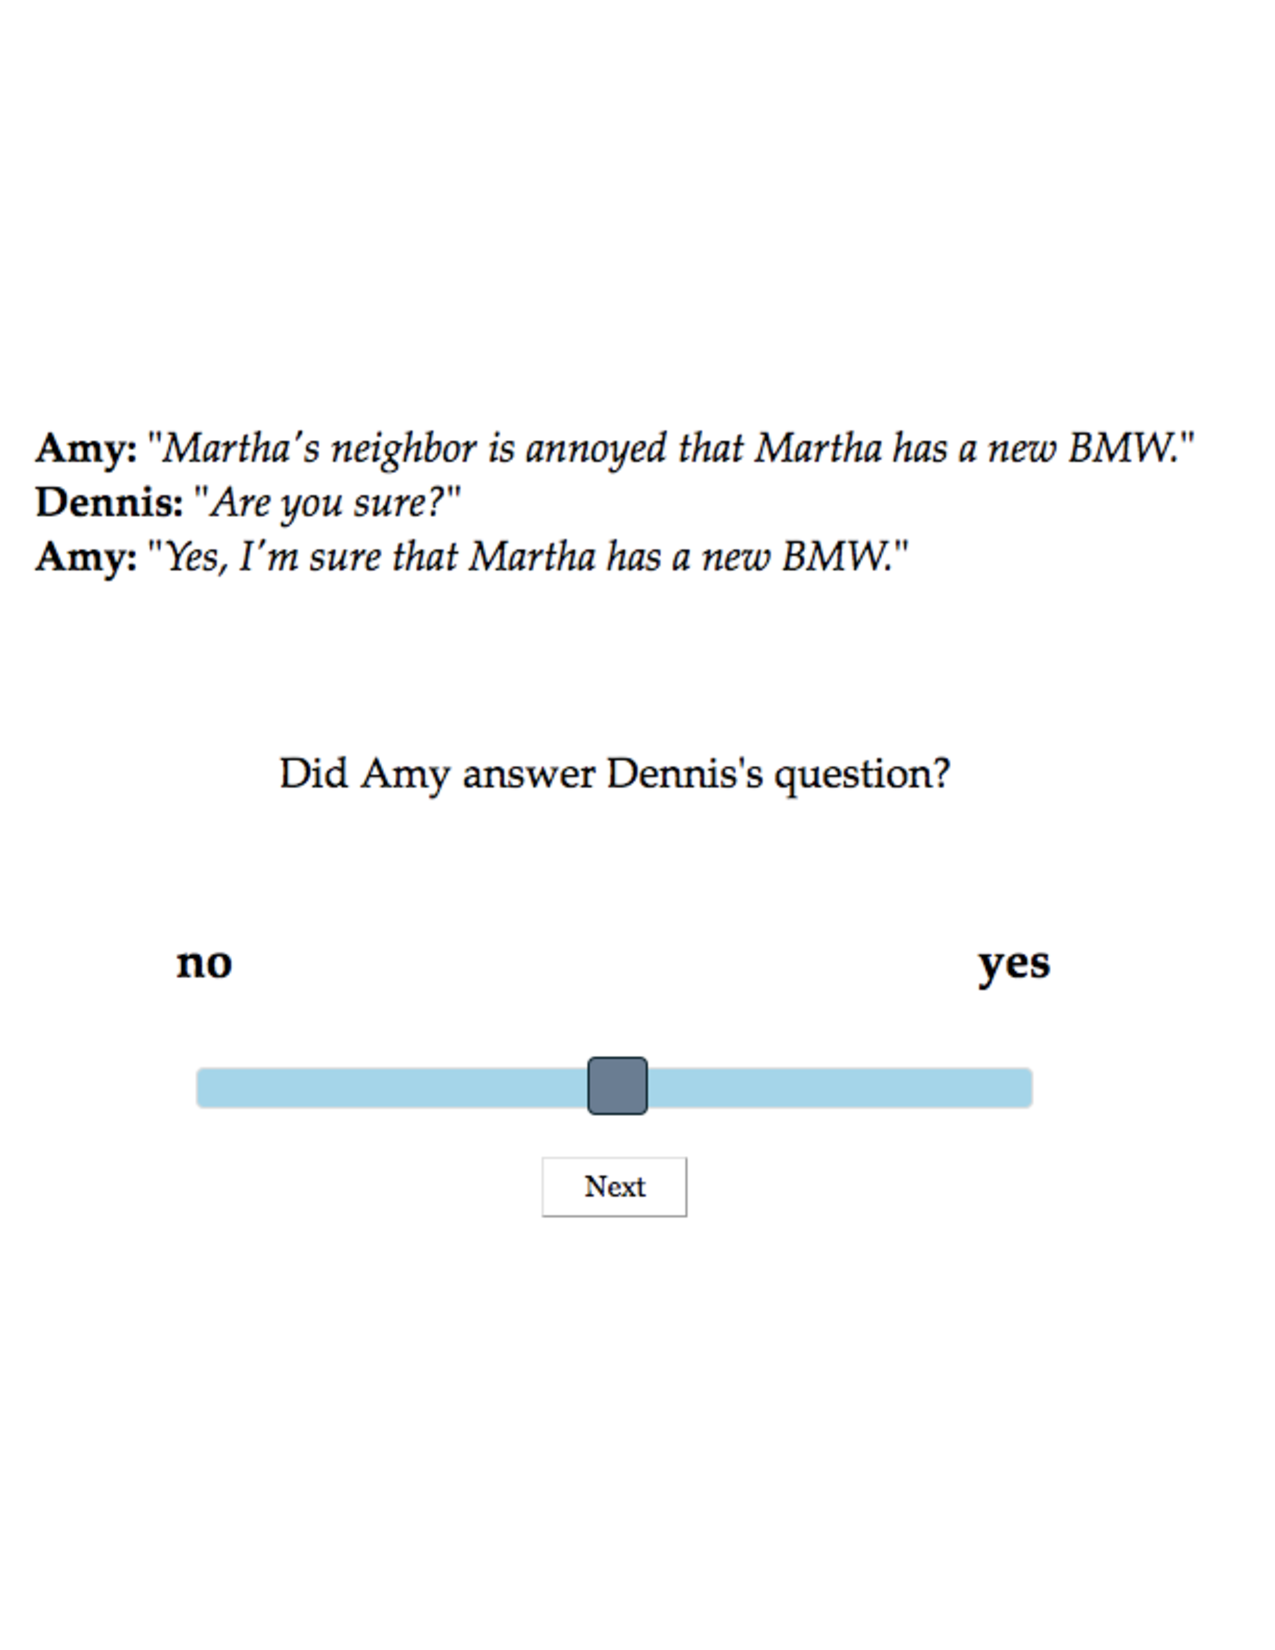
\includegraphics[width=8cm]{exp2-trial}
\end{center}
\caption{A sample trial in experiments 2a and 2b}\label{f-trial-exp2}
\end{figure}

\subsubsection{Analysis}

The data from 6 participants who did not self-identify as native speakers of American English were excluded. As with Exps 1a and 2a, participants' responses were recoded so that a `yes' (1) response means that the relevant content is not at-issue.

\paragraph{Responses to control stimuli.} 
Inspection of the response means of the remaining 244 participants to six main clause control stimuli revealed 6 participants whose response means were more than 3 standard deviations above the group mean (which was 0.04). Further inspection revealed that these participants' responses to the control questions were systematically higher than the group means and involved 14 of the 17 projective contents, suggesting that these participants did not attend to the task or interpreted the task differently. The data from these 6 participants were also excluded, leaving data from 238 participants (ages 20-77; median: 30). 

\subsubsection{Results}

The boxplots in Figure \ref{f-exp2a} illustrate the not-at-issueness of the nine expression/content pairs, which are again are ordered by their mean (given by the blue dots), with the expression/content pairs with the lowest not-at-issueness on the left. 

\begin{figure}[!h]

\begin{center}

\includegraphics[width=12cm]{/Users/judith/Documents/current-research-topics/NSF-NAI/prop-att-experiments/1factive-verbs/5-NAI/results/graphs/boxplot-not-at-issueness}
\end{center}

\caption{Boxplots of responses to nine expression/content pairs in {\em Are you sure?}-diagnostic; the blue dots show the mean responses}\label{f-exp2a}
\end{figure}

\begin{itemize}

\item {\tt nai.1} shows that all contents significantly more NAI than main clauses

\item {\tt comp\_nai} shows that significant differences among contents

only, stop, stupid, discover, know $<$ annoyed

discover $<$ know, NomApp, NRRC, possNP

stop, stupid $<$ discover 

stupid, only $<$ know $<$ NomApp, NRRC, possNP

only, stop, stupid $<$ NomApp

only, possNP, stop $<$ NRRC

only $<$ possNP, only, stupid

stop, stupid $<$ possNP

\item Correlation of the two not-at-issueness diagnostics:

\begin{figure}[!h]

\begin{center}

\includegraphics[width=16.5cm]{/Users/judith/Documents/current-research-topics/NSF-NAI/prop-att-experiments/1factive-verbs/5-NAI/results/graphs/correlation-means-NAI-NAI}
\end{center}

\caption{Correlation of the means of the two not-at-issueness diagnostics (Experiments 1a and 2a)}\label{f-corr1}
\end{figure}


\item Correlation of projectivity with the new not-at-issueness diagnostic:

\begin{figure}[!h]

\begin{center}

\includegraphics[width=16.5cm]{/Users/judith/Documents/current-research-topics/NSF-NAI/prop-att-experiments/1factive-verbs/5-NAI/results/graphs/correlation-means-NAI-NAI-Proj}
\end{center}

\caption{Correlation of the mean projectivity with the two not-at-issueness diagnostics (Experiments 1a and 2a)}\label{f-corr2}
\end{figure}

\end{itemize}


\subsubsection{Discussion}

\subsection{Experiment 2b} 

\subsubsection{Methods}

\paragraph{Participants.} 250 participants with U.S.\ IP addresses and at least 97\% of previous HITs approved were recruited on Amazon's Mechanical Turk platform. They were paid 30 cents for their participation.

\paragraph{Materials.} The target stimuli in this experiment consisted of 3-turn discourses between two individuals, as illustrated in (\ref{sure}). The same twelve trigger/content pairs as in Experiment 1b (see (\ref{examples-1b})) were realized with the same 20 contents, yielding a total of 240 indicative sentences, which were realized as the first individual's first utterance. In contrast to Experiment 1b, the target stimuli in this experiment were indicative sentences in which the triggers were not embedded under an entailment canceling operator, as illustrated for nominal appositives and {\em know} in A's first utterances in (\ref{sure}). The second turn of the stimuli consisted of a different person uttering {\em Are you sure?}. The third turn consisted of the first person uttering {\em Yes, I am sure that}, with the relevant content realized as the content of the complement of {\em sure}. As in Experiment 1b, an additional 20 control stimuli were formed from the 20 contents: here, person A uttered a main clause conveying such a content (e.g., {\em A: Raul was drinking chamomile tea. B: Are you sure? A: Yes, I am sure that Raul was drinking chamomile tea.}).

As in Experiment 1b, a set of 20 stimuli was randomly created for each participant from 20 distinct contents so that each set included twelve stimuli formed with the twelve attitude predicates and eight control stimuli.


\paragraph{Procedure.} The procedure was the same as in experiment 2a, described in section \ref{s-methods-2a}, except that participants responded to 20 stimuli (rather than just 15).

\subsubsection{Analysis}

The data from 6 participants who did not self-identify as native speakers of American English were excluded. As with the previous experiments, participants' responses were recoded so that a `yes' (1) response means that the relevant content is not at-issue.

\paragraph{Responses to control stimuli.} 
Inspection of the response means of the remaining 244 participants to eight main clause control stimuli revealed 6 participants whose response means were more than 3 standard deviations above the group mean (which was 0.05). Further inspection revealed that these participants' responses to the control questions were systematically higher than the group means and involved 18 of the 20 contents, suggesting that these participants did not attend to the task or interpreted the task differently. The data from these 6 participants were also excluded, leaving data from 238 participants (ages 18-77; median: 30). 

\subsubsection{Results}

The boxplots in Figure \ref{f-exp2b} illustrate the not-at-issueness of the contents of the complements of the twelve factive predicates, which are again are ordered by their mean (given by the blue dots), with the factive predicate whose complement was least not-at-issue on the left.

\begin{figure}[!h]

\begin{center}

\includegraphics[width=16.5cm]{/Users/judith/Documents/current-research-topics/NSF-NAI/prop-att-experiments/1factive-verbs/7-NAI-factive-verbs/results/graphs/boxplot-not-at-issueness}
\end{center}

\caption{Boxplots of responses to the contents of the complements of the twelve attitude predicates in {\em Are you sure?}-diagnostic; the blue dots show the mean responses}\label{f-exp2b}
\end{figure}

\begin{figure}[!h]

\begin{center}

\includegraphics[width=16.5cm]{/Users/judith/Documents/current-research-topics/NSF-NAI/prop-att-experiments/1factive-verbs/7-NAI-factive-verbs/results/graphs/correlation-means-NAI-NAI}
\end{center}

\caption{Correlation of the means of the two not-at-issueness diagnostics (Experiments 1b and 2b)}\label{f-corr3}
\end{figure}

Correlation of projectivity with the new not-at-issueness diagnostic:

\begin{figure}[!h]

\begin{center}

\includegraphics[width=16.5cm]{/Users/judith/Documents/current-research-topics/NSF-NAI/prop-att-experiments/1factive-verbs/7-NAI-factive-verbs/results/graphs/correlation-means-NAI-NAI-Proj}
\end{center}

\caption{Correlation of the mean projectivity with the two not-at-issueness diagnostics (Experiments 1b and 2b)}\label{f-corr4}
\end{figure}

\subsubsection{Discussion}

\section{Discussion}\label{s5}

\begin{itemize}

\item Other refs on ps: \citealt{schwarz07,chemla09,tiemann-etal11}. \citealt{zeevat92} distinguishes resolution and lexical triggers based on whether they can be globally accommodated; see \citealt{amaral-cummins2015} for experimental investigation of that difference.

\item These experimental findings provide empirical support for Simons et al's projection hypothesis. Furthermore, they constitute a problem for accommodation-based theories of presupposition projection: since the minimal discourse context in which the stimuli in Exp 1a were presented does not license local accommodation, such theories wrongly predict robust presupposition projection, i.e., cannot account for the observed projection variability.

\end{itemize}

\appendix

\section{Experiment 1a/2a stimuli}\label{a-exp1a-2a-stimuli}

The polar questions used in Experiment 1a are given below grouped by the content that constituted the projective content. This also makes it possible to see which trigger/content pairs had overlap with which other ones. Experiment 2a used main clause versions of these polar questions. 

\begin{enumerate}

\item  "muffins": \\
     Content:"these muffins have blueberries in them",\\
     "MC":"Do these muffins have blueberries in them?",\\
     "NRRC":"Are these muffins, which have blueberries in them, gluten-free and low-fat?",\\
     "only":"Do these muffins only have blueberries in them?"

\item "pizza": \\
     Content:"this pizza has mushrooms on it",\\
     "MC":"Does this pizza have mushrooms on it?",\\
     "only":"Does this pizza only have mushrooms on it?",\\
     "annoyed":"Is Sam annoyed that this pizza has mushrooms on it?",\\
     "discover":"Did Sam discover that this pizza has mushrooms on it?"

\item "play": \\
     Content:"Jack was playing outside with the kids",\\
     "MC":"Was Jack playing outside with the kids?",\\
     "stop":"Did Jack stop playing outside with the kids?",\\
     "know":"Does Daria know that Jack was playing outside with the kids?",\\
     "discover":"Did Paula discover that Jack was playing outside with the kids?"

\item "veggie": \\
     Content:"Don is a vegetarian",\\
     "NomApp":"Is Don, a vegetarian, going to find something to eat here?",\\
     "NRRC":"Is Don, who is a vegetarian, going to find something to eat here?",\\
     "MC":"Is Don a vegetarian?"

\item "cheat": \\
     Content:"Raul cheated on his wife",\\
     "MC":"Did Raul cheat on his wife?",\\
     "know":"Does Daria know that Raul cheated on his wife?",\\
     "stupid":"Was Raul stupid to cheat on his wife?"

\item "nails": \\
     Content:"Mary's daughter has been biting her nails",\\
     "MC":"Has Mary's daughter been biting her nails?",\\
     "discover":"Did Mary discover that her daughter has been biting her nails?",\\
     "stop":"Has Mary's daughter stopped biting her nails?",\\
     "stupid":"Is Mary's daughter stupid to be biting her nails?"

\item  "ballet": \\
     Content:"Ann used to dance ballet",\\
     "MC":"Did Ann use to dance ballet?",\\
     "NomApp":"Is Ann, a former ballet dancer, limping?",\\
     "stop":"Did Ann stop dancing ballet?"

\item "kids": \\
     Content:"John's kids were in the garage",\\
     "only":"Were John's kids only in the garage?",\\
     "MC":"Were John's kids in the garage?",\\
     "stupid":"Were John's kids stupid to be in the garage?"

\item "hat": \\
     Content:"Samantha has a new hat",\\
     "MC":"Does Samantha have a new hat?",\\
     "possNP":"Was Samantha's new hat expensive?",\\
     "know":"Does Daria know that Samantha has a new hat?",\\
     "annoyed":"Is Joyce annoyed that Samantha has a new hat?"

\item "bmw": \\
     Content:"Martha has a new BMW",\\
     "MC":"Does Martha have a new BMW?",\\
     "possNP":"Was Martha's new BMW expensive?",\\
     "NomApp":"Was Martha's new car, a BMW, expensive?",\\
     "annoyed":"Is Martha's neighbor annoyed that Martha has a new BMW?",\\
     "know":"Does Billy know that Martha has a new BMW?"

\item "boyfriend": \\
     Content:"Betsy has a boyfriend",\\
     "MC":"Does Betsy have a boyfriend?",\\
     "NRRC":"Is Betsy, who has a boyfriend, flirting with the neighbor?",\\
     "possNP":"Is Betsy's boyfriend from around here?"

\item "alcatraz": \\
     Content:"Mike visited Alcatraz",\\
     "MC":"Did Mike visit Alcatraz?",\\
     "NRRC":"Is Mike, who visited Alcatraz, a history fan?",\\
     "discover":"Did Jane discover that Mike visited Alcatraz?",\\
     "know":"Does Jane know that Mike visited Alcatraz?"

\item "aunt": \\
     Content:"Janet has a sick aunt",\\
     "MC":"Does Janet have a sick aunt?",\\
     "NRRC":"Is Janet, who has a sick aunt, very compassionate?",\\
     "know":"Does Melissa know that Janet has a sick aunt?",\\
     "possNP":"Has Janet's sick aunt been recovering?"

\item "cupcakes": \\
     Content:"Marissa brought the cupcakes",\\
     "MC":"Did Marissa bring the cupcakes?",\\
     "NRRC":"Is Marissa, who brought the cupcakes, a good baker?",\\
     "know":"Does Max know that Marissa brought the cupcakes?",\\

\item "soccer": \\
     Content:"the soccer ball has a hole in it",\\
     "MC":"Does the soccer ball have a hole in it?",\\
     "NRRC":"Was the soccer ball, which has a hole in it, a gift from Uncle Bill?",\\
     "annoyed":"Is Mandy annoyed that the soccer ball has a hole in it?",\\
     "discover":"Did Mandy discover that the soccer ball has a hole in it?",\\
     "know":"Does Mandy know that the soccer ball has a hole in it?"

\item "olives": \\
   	Content:"this bread has olives in it",\\
   	"MC":"Does this bread have olives in it?",\\
   	"annoyed":"Is Barbara annoyed that this bread has olives in it?",\\

\item "stuntman": \\
   	Content:"Richie is a stuntman",\\
   	"MC":"Is Richie a stuntman?",\\
   	"NomApp":"Did Richie, a stuntman, break his leg?",\\
   	"stupid":"Is Richie stupid to be a stuntman?"

\end{enumerate}

\bibliographystyle{cslipubs-natbib}
\bibliography{bibliography}


\end{document}
